\chapter{General Guidelines for Optimizing the Physical Data Layout and Query Processor in GDBMSs}
\label{c:guidelines}

In this section, we review the primary components that form the storage layers of \gls{gdbms}s, the system's primary operators, and the general data access patterns of these operators when evaluating a query. We then draw a basic set of guidelines that will instruct the design of the physical data layout and query-processing techniques introduced in later chapters.

Section \ref{sec:property-graph-data-model} briefly describes the \emph{property graph data model}. Section \ref{sec:storage-components} describes the primary storage components of \gls{gdbms}s that adopt the property graph data model, while Section \ref{sec:operators} reviews the query processing operators in \gls{gdbms}s. We end the chapter by stating our guidelines in Section \ref{sec:guidelines}.

\section{Property Graph Data Model}
\label{sec:property-graph-data-model}

\begin{figure}
	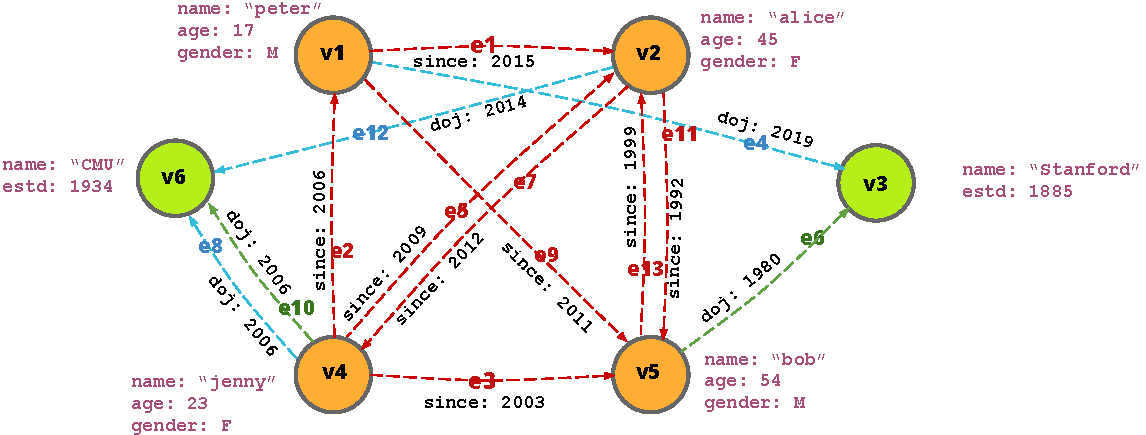
\includegraphics[scale=0.86]{img/property-graph}
	\vspace{-8pt}
	\caption{Running example graph.}
	\label{fig:runn}
	\vspace{-8pt}
\end{figure}

Figure~\ref{fig:runn} shows a graph data in the property graph data model. A property graph consists \emph{vertices} that represent entities and directed \emph{edges} between vertices that represent relationships between entities. Each vertex and edge has a particular \emph{label}, describing the high-level categories of vertices and edges. For example, in Fig.~\ref{fig:runn}, vertices have labels: \texttt{PERSON} and \texttt{ORG}, while edges have labels: \texttt{FOLLOWS}, \texttt{WORKAT} and \texttt{STUDYAT}.

Similar to columns in relational tables, vertices and edges can have (key, value) \emph{properties}. Although the properties of vertices and edges do not need to adhere to a strict \emph{schema }, in practice many of these properties will be highly structured, i.e., similar set of properties will exist on vertices and edges of the same label.

\section{Primary Storage Components in GDBMSs}
\label{sec:storage-components}

In every \gls{gdbms} we are aware of, the edges of a graph are stored in data structure called \emph{adjacency lists}. An adjacency list of a vertex is a map to a vertex's direct set of \emph{adjacent} edges and \emph{neighbouring} vertices. In a \gls{gdbms}, each vertex has 2 adjacency lists - a \emph{forward adjacency list} containing outward edges of that vertex, and a \emph{backward adjacency list} that holds inward edges of the vertex. One can think of edges in the graph as a relational table, having 3 attributes, a source vertex, a destination vertex and an \texttt{edgeID}. The adjacency lists can then be thought of as an \emph{index} on this relational table that is \emph{clustered} by either the source or destination vertex. In practice, often this index has depth of 1 or 2, so given a vertex, a system can access its list of edges in 1 or 2 lookups. By having adjacency lists of a vertex $u$ in either direction, the system can access the list of outward and inward edges and neighbouring vertices of $u$ directly in a constant-time lookup operation, which provides the core capability of fast joins to a \gls{gdbms}. 

Typically, a single-directional adjacency list of vertex $u$ is further clustered into sublists by the edge label of the edges. This enables extending a vertex through its edges with a \emph{particular} label in constant time. The rationale behind the sub-clustering is that many queries by applications have specific label on query edges. Some systems further order the edge in the adjacency lists either by a property of adjacent edge or neighbour vertex or simply by neighbour vertex. Sorting enables the system to access parts of list in time logarithmic in the size of the adjacency list.

A \gls{gdbms} also stores properties that appear on the vertices and the edges. There are multiple solutions for storing properties. The most straightforward approach is to store properties in a \emph{key-value store} \cite{dgraph} and referenced by the attribute key and the \texttt{vertexID} or \texttt{edgeID}. Properties can also be stored as a \emph{variable-sized} byte-encoded record of each vertex or edge in the same manner as row-oriented \gls{rdbms} stores tuples. A record is considered variable-sized because the number of properties on an entity is not fixed. Searching for a property in variable-sized records involves decoding and parsing the entire record until the matching attribute is found, which can be very slow. Also, the addition and deletion of properties are not straightforward in records. Yet another way of storing properties is in a doubly linked-list, as in Neo4j \cite{neo4j}, that makes additions and deletions easy though searching is still a linear-time operation.

\section{Query Execution in GDBMSs}
\label{sec:operators}

In this section, we review the general execution of queries in a \gls{gdbms} by analyzing major operators used in the query plans. Though systems differ in their architectures and implementation of operators that they support, there still remains a similarity in their data access patterns. We use the Cypher query language \cite{cypher} to describe the queries to a \gls{gdbms}. A user query typically consists of 3 parts, 1) a \texttt{MATCH} clause with a subgraph query pattern $Q(V_Q, E_Q)$, where $V_Q$ and $E_Q$ are the query vertex and edge variables, that is matched to the input graph's topology; 2) \texttt{WHERE} claue that contains a predicate $\rho$ over properties of edge and vertex variable that the matched subgraph must satisfy; and 3) a \texttt{RETURN} statement that returns a projection of matches in the graph or its aggregated value. Example \ref{ex:cypher-example} shows a typical query written in Cypher language, to query the example graph in figure~\ref{fig:runn}.

\begin{example}
	\label{ex:cypher-example}
	Consider the following query Q. 
	{\em 
		\begin{lstlisting}[numbers=none,  showstringspaces=false,belowskip=0pt ]
		MATCH (a:PERSON)$-$[e:WORKAT]$\rightarrow$(b:ORG)
		WHERE a.age $>$ 22 AND b.estd < 2015
		RETURN *\end{lstlisting}
	}
	This query returns all the PERSON vertices and their workplaces, constrained to the condition that the \textsc{\char13}\texttt{age}\textsc{\char13} property of PERSON vertex has a value that is greater than 22 and \textsc{\char13}\texttt{established}\textsc{\char13} property of ORG vertex is less than 2015. a and b are query vertex variables while e is a query edge variable.
\end{example}
\vspace{-5pt}

The following are the major operators used for matching the subgraph pattern and evaluating predicates in a query.
\begin{itemize}
	
	\item \textbf{\texttt{SCAN}}: Scans a set of vertices and edges from the graph topology.
	
	\item \textbf{\texttt{NEIGHBOURHOOD JOIN}}: e.g. \texttt{EXTEND/INTERSECT} in Graphflow, \texttt{EXPAND} in Neo4j. On a high level, the neighbourhood join operator matches the subgraph query pattern $Q$, one vertex variable at a time. The input to the operator is a partial $k$-match, $t$, of $Q$. We define a partial $k$-match of $Q$ as a set of vertices from the input graph assigned to the projection of $Q$ onto the set of $k$ query vertex variables. For each partially matched $t$, the operator extends $t$ by matching an unmatched query vertex, say $v$, such that there is atleast one edge in $E_Q$ between $v$ and $t$'s vertices' variables. The \emph{join} happens by sequentially reading adjacent edges and neighbour vertices from (forward/backward) adjacency list of one or more matched vertices of $t$, to produce a $k+1$-match.

	\item \textbf{\texttt{PROPERTY READER}}: (Vertex/Edge) property reader reads a property value of any vertex or edge that has been assigned to a variable in $V_Q$ or $E_Q$ of a partial match $t$, from the underlying properties storage. 

	\item \textbf{\texttt{FILTER}}: Given the predicate $\rho$ from the \texttt{WHERE} clause of the query and a partial match, $t$, of $Q$, the \texttt{FILTER} operator omits $t$ from the result of the query if $t$ does not pass the predicate $\rho$.
	
\end{itemize}

\begin{figure}
	\hfill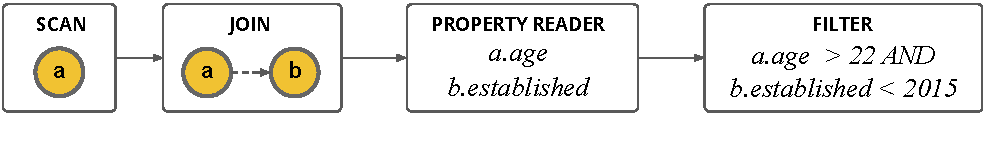
\includegraphics[scale=0.80]{img/ex-qp}\hfill
	\vspace{-8pt}
	\caption{Query plan for Example~\ref{ex:cypher-example}.}
	\label{fig:ex-qp}
	\vspace{-8pt}
\end{figure}

Figure~\ref{fig:ex-qp} shows one of the query plans that the system will generate to execute query in Example~\ref{ex:cypher-example}. It consists of the following sequence of operators: 1) \texttt{SCAN} operator that matches the variable $a$ in query to vertex in the graph having label \texttt{PERSON}, 2) \texttt{JOIN} operator matches $b$ by reading the forward adjacency list of $a$'s match, 3) \texttt{PROPERTY READER} reads the properties \texttt{age} and \texttt{estd} of $a$'s and $b$'s match, and 4) \texttt{FILTER} operators filters out the matched query pattern that do not confrm to the constraint $a.age > 22$ $AND$ $b.estd < 2015$.

\section{Guidelines}
\label{sec:guidelines}

We next outline a set of guidelines for designing the physical data layout and query processor of a \gls{gdbms}.

\begin{guideline}[Edges are doubly-indexed.]
Each edge appears in the forward adjacency list of that edge's source vertex and the backward adjacency list of it's destination vertex. This results in a 2x replication factor in storing the topology of a graph in the system. This  replication cannot be avoided by dropping an adjacency list in any one direction without hampering the capability to perform fast neighbour joins, which is one of the core feature of \gls{gdbms}s.
\end{guideline}

\label{ssec:edges-ordered}
\begin{guideline}[Edge properties are read in the same order as edges in an adjacency list.]
	
During the execution of a query, the \texttt{JOIN} operator will access the edges of a vertex $v$ in the order these edges appear in $v$'s (forward/backward) adjacency lists. Note that the edge or its property might not be read in consecutive operations, hence we do not call the access \emph{sequential}; nevertheless, ordering is preserved. If the query also needs to access the properties of these edges, the access to these edge properties will also be in the same order in which edges were read from the adjacency list. 

This raises the question of whether we can also read edges and edge properties sequentially from the memory at once and hence benefit from the cache locality available at hand. This can be achieved by organizing the edge propreties into lists in an order identical to that of edges in the adjacency list. Since, each edge appears twice, each edge property has to be replicated twice in the system. This might be quite expensive because every property and not just the edge and neighbour vertex need to be replicated. In addition, if the edges in the adjacency lists are sorted, as is done in some of the systems, then the list of ordered edge properties also needs to be kept in sorted order. This makes updates to the system costly, since an insertion of a new edge in between the adjacency list will effect the ordering of all the edge's property lists.

\end{guideline}

\begin{guideline}[Vertices cannot be ordered to make access from all neighbour verteices sequential.]
\label{gdln:vertices-unordered}

Contrary to how the edges and edge properties can be strictly ordered for each of the adjacency lists, there cannot be an ordering on the vertices that localizes the access to neighbour vertices of every vertex and to the properties of these neighbour vertices without prohibitive data replication. In general, if a vertex $v$ has $n$ neighours, then $v$ and its properties need to be replicated $n$ times. Hence, localizing access to neighbour vertices and their properties should not be put in the desiderata of the system's physical data layout design.

\end{guideline}

\begin{guideline}[Graph data often has partial structure.]
\label{gdln:graph-schema}
Even though the property graph data model is semi-structured, in practise many graph databases stored in \gls{gdbms}s have structure in different components, which \gls{gdbms}s can exploit. One reason this structure exist is that, as observed by prior works \cite{survey}, often the data in \gls{gdbms} comes from structured data in \gls{rdbms}. Infact, several of the \gls{gdbms} providers from the industry and some academics are actively working of defining a schema language for the property graph data model \cite{schema-validation-bonifati, defining-schema-hartig}. We identify three commonly appearing structure in property graph data:

\begin{enumerate}
	
	\item Often, edge labels in the graph data have a well-defined set of source and destination vertex label(s). This restricts the vertices to  having inward or outward edges of only a definite set of labels. For example, in the LDBC social network benchmark \cite{ldbc}, edges having label KNOWS only exists between vertices of label PERSON.
	\label{gdln:graph-schema-rule1}
	
	\item The number of edges of a particular label to which a source or destination vertex can be associated, is a property of the edge label. We call this the \emph{cardinlaity} of an edge label. \emph{One-to-one} cardinality means that there can only be single edge of a particular label from a source vertex and to a destination vertex. \emph{Many-to-one} permits a single edge of a label from a source vertex but multiple edges to a destination vertex. Similar analogy can be applied to \emph{one-to-many} and \emph{many-to-many} cardinality edge labels too.
	\label{gdln:graph-schema-rule2}
	
	\item Similar to the attributes of a relational table, properties on an edge or vertex and the datatypes of these properties can \emph{often} be determined by its edge or vertex label. For example, a vertex of label PERSON in LDBC SNB has the following properties: firstName:\texttt{STRING}, lastName: \texttt{STRING}, gender:\texttt{INT} etc., that occurs on all the vertices of label PERSON. As long as a significant fraction of vertices and edges with a particular label have a common set of properties, a system can exploit this structuredness to store these properties more efficiently. 
	
\end{enumerate}

Such structure in data provides an opportunity to design more efficient and simpler data structures for accessing the storage layer of \gls{gdbms}. However, not all data in graph databases has structure. As a working terminology, we will use the following terms:

\begin{itemize}
	\item \textbf{Structured/unstructured edge:} An edge of a particular label, that follows above-mentioned points \ref{gdln:graph-schema-rule1} and \ref{gdln:graph-schema-rule2}, is called an structured edge. An edge that is not structured, is called an unstructured edge.
	 
	\item \textbf{Structured/unstructured property:} A structured property is a property on a vertex or edge that, 1) can be determined by the vertex type or edge label of that entity; 2) appears in a significant fraction of the vertices of edges of a particular label; and 3) have the same data type in all its occurrence. Any property that is not a structured poperty, is considered unstructed.
	
\end{itemize}

We focus on optimizing the storage of structured part of the graph data in this thesis. It forms an interesting research topic to optimize a system for unstructured part of graph data. A standard approach is to serialize the key, datatype and value of each property  of our work on structured properties. Owing to the erratic nature of unstructured properties, storing them in variable-length records or linked-list as (attribute, value) pairs is a viable solution. Structured property storage can, however, be optimized to benefit memory footprint as well as access performance.

\end{guideline}

\begin{guideline}[Queries read a small subset of the vertex or edge properties]
In order to understand the nature of queries user ask on \gls{gdbms}, we conducted a survey of 100 StackOverflow questions containing openCypher queries. We focused on queries of analytical nature and discards transactional ones like insert, delete and update. We observe the following: 

\begin{itemize}
	
	\item Out of the 100 queries, 68 accessed at least one of the properties on a vertex or an edge. Of these, 61 accesses vertex properties and 13 accesses edge properties.
	
	\item Only 11 queries returned all the properties of a query edge or vertex, while 35 of them return specific properties.
	
	\item Average number of properties accessed by those queries that explicitly return a set of properties is only 1.6.
	
\end{itemize}

We can observe that conclude that vertex properties are more popularly accessed as compared to edge properties and most of the queries only access 1 or at most 2 properties.

\end{guideline}
